% Options for packages loaded elsewhere
\PassOptionsToPackage{unicode}{hyperref}
\PassOptionsToPackage{hyphens}{url}
\PassOptionsToPackage{dvipsnames,svgnames,x11names}{xcolor}
%
\documentclass[
  letterpaper,
  DIV=11,
  numbers=noendperiod]{scrreprt}

\usepackage{amsmath,amssymb}
\usepackage{iftex}
\ifPDFTeX
  \usepackage[T1]{fontenc}
  \usepackage[utf8]{inputenc}
  \usepackage{textcomp} % provide euro and other symbols
\else % if luatex or xetex
  \usepackage{unicode-math}
  \defaultfontfeatures{Scale=MatchLowercase}
  \defaultfontfeatures[\rmfamily]{Ligatures=TeX,Scale=1}
\fi
\usepackage{lmodern}
\ifPDFTeX\else  
    % xetex/luatex font selection
\fi
% Use upquote if available, for straight quotes in verbatim environments
\IfFileExists{upquote.sty}{\usepackage{upquote}}{}
\IfFileExists{microtype.sty}{% use microtype if available
  \usepackage[]{microtype}
  \UseMicrotypeSet[protrusion]{basicmath} % disable protrusion for tt fonts
}{}
\makeatletter
\@ifundefined{KOMAClassName}{% if non-KOMA class
  \IfFileExists{parskip.sty}{%
    \usepackage{parskip}
  }{% else
    \setlength{\parindent}{0pt}
    \setlength{\parskip}{6pt plus 2pt minus 1pt}}
}{% if KOMA class
  \KOMAoptions{parskip=half}}
\makeatother
\usepackage{xcolor}
\setlength{\emergencystretch}{3em} % prevent overfull lines
\setcounter{secnumdepth}{5}
% Make \paragraph and \subparagraph free-standing
\makeatletter
\ifx\paragraph\undefined\else
  \let\oldparagraph\paragraph
  \renewcommand{\paragraph}{
    \@ifstar
      \xxxParagraphStar
      \xxxParagraphNoStar
  }
  \newcommand{\xxxParagraphStar}[1]{\oldparagraph*{#1}\mbox{}}
  \newcommand{\xxxParagraphNoStar}[1]{\oldparagraph{#1}\mbox{}}
\fi
\ifx\subparagraph\undefined\else
  \let\oldsubparagraph\subparagraph
  \renewcommand{\subparagraph}{
    \@ifstar
      \xxxSubParagraphStar
      \xxxSubParagraphNoStar
  }
  \newcommand{\xxxSubParagraphStar}[1]{\oldsubparagraph*{#1}\mbox{}}
  \newcommand{\xxxSubParagraphNoStar}[1]{\oldsubparagraph{#1}\mbox{}}
\fi
\makeatother


\providecommand{\tightlist}{%
  \setlength{\itemsep}{0pt}\setlength{\parskip}{0pt}}\usepackage{longtable,booktabs,array}
\usepackage{calc} % for calculating minipage widths
% Correct order of tables after \paragraph or \subparagraph
\usepackage{etoolbox}
\makeatletter
\patchcmd\longtable{\par}{\if@noskipsec\mbox{}\fi\par}{}{}
\makeatother
% Allow footnotes in longtable head/foot
\IfFileExists{footnotehyper.sty}{\usepackage{footnotehyper}}{\usepackage{footnote}}
\makesavenoteenv{longtable}
\usepackage{graphicx}
\makeatletter
\newsavebox\pandoc@box
\newcommand*\pandocbounded[1]{% scales image to fit in text height/width
  \sbox\pandoc@box{#1}%
  \Gscale@div\@tempa{\textheight}{\dimexpr\ht\pandoc@box+\dp\pandoc@box\relax}%
  \Gscale@div\@tempb{\linewidth}{\wd\pandoc@box}%
  \ifdim\@tempb\p@<\@tempa\p@\let\@tempa\@tempb\fi% select the smaller of both
  \ifdim\@tempa\p@<\p@\scalebox{\@tempa}{\usebox\pandoc@box}%
  \else\usebox{\pandoc@box}%
  \fi%
}
% Set default figure placement to htbp
\def\fps@figure{htbp}
\makeatother

\pagenumbering{gobble} % Tar bort sidnummer på framsidan
\usepackage[hyphens]{url}
\usepackage{hyperref}
\urlstyle{same}
\KOMAoption{captions}{tableheading}
\makeatletter
\@ifpackageloaded{bookmark}{}{\usepackage{bookmark}}
\makeatother
\makeatletter
\@ifpackageloaded{caption}{}{\usepackage{caption}}
\AtBeginDocument{%
\ifdefined\contentsname
  \renewcommand*\contentsname{Innehållsförteckning}
\else
  \newcommand\contentsname{Innehållsförteckning}
\fi
\ifdefined\listfigurename
  \renewcommand*\listfigurename{Figurförteckning}
\else
  \newcommand\listfigurename{Figurförteckning}
\fi
\ifdefined\listtablename
  \renewcommand*\listtablename{Tabellförteckning}
\else
  \newcommand\listtablename{Tabellförteckning}
\fi
\ifdefined\figurename
  \renewcommand*\figurename{Figur}
\else
  \newcommand\figurename{Figur}
\fi
\ifdefined\tablename
  \renewcommand*\tablename{Tabell}
\else
  \newcommand\tablename{Tabell}
\fi
}
\@ifpackageloaded{float}{}{\usepackage{float}}
\floatstyle{ruled}
\@ifundefined{c@chapter}{\newfloat{codelisting}{h}{lop}}{\newfloat{codelisting}{h}{lop}[chapter]}
\floatname{codelisting}{Lista}
\newcommand*\listoflistings{\listof{codelisting}{Listförteckning}}
\makeatother
\makeatletter
\makeatother
\makeatletter
\@ifpackageloaded{caption}{}{\usepackage{caption}}
\@ifpackageloaded{subcaption}{}{\usepackage{subcaption}}
\makeatother

\ifLuaTeX
\usepackage[bidi=basic]{babel}
\else
\usepackage[bidi=default]{babel}
\fi
\babelprovide[main,import]{swedish}
% get rid of language-specific shorthands (see #6817):
\let\LanguageShortHands\languageshorthands
\def\languageshorthands#1{}
\usepackage{bookmark}

\IfFileExists{xurl.sty}{\usepackage{xurl}}{} % add URL line breaks if available
\urlstyle{same} % disable monospaced font for URLs
\hypersetup{
  pdftitle={R Programmering},
  pdfauthor={Peter Lantz},
  pdflang={sv},
  colorlinks=true,
  linkcolor={blue},
  filecolor={Maroon},
  citecolor={Blue},
  urlcolor={Blue},
  pdfcreator={LaTeX via pandoc}}


\title{R Programmering}
\author{Peter Lantz}
\date{2025-04-23}

\begin{document}
\maketitle

\renewcommand*\contentsname{Innehållsförteckning}
{
\hypersetup{linkcolor=}
\setcounter{tocdepth}{2}
\tableofcontents
}

\bookmarksetup{startatroot}

\chapter*{}\label{section}
\addcontentsline{toc}{chapter}{}

\markboth{}{}

\bookmarksetup{startatroot}

\chapter*{Abstrakt}\label{abstrakt}
\addcontentsline{toc}{chapter}{Abstrakt}

\markboth{Abstrakt}{Abstrakt}

The aim of this project was to investigate whether a relatively simple
linear regression model could predict car prices with a coefficient of
determination (R²) of at least 0.80 using only two or three predictors.
Data was collected from Blocket.se, and three different models were
trained. All models achieved an R² greater than 0.80. Since the goal was
to keep the model simple, the best-performing model was not selected.
Instead, a model with fewer predictors was chosen, which still
demonstrated strong predictive performance. The results show that a
straightforward model can effectively estimate car prices for new
observations, thereby fulfilling the objectives of the study.

\bookmarksetup{startatroot}

\chapter{Inledning}\label{inledning}

\pagenumbering{arabic}

\section{Bakgrund}\label{bakgrund}

I dagens samhälle är vi allt mer beroende av transporter för att kunna
uppfylla våra dagliga åtaganden -- arbete, inköp, fritidsaktiviteter och
familjelogistik. Trots att det finns andra transportalternativ upplever
många bilen som ett bekvämt och flexibelt val, eftersom den erbjuder
kontroll och oberoende.

Denna utveckling återspeglas i antalet personbilar i trafik, som enligt
Figur~\ref{fig-trafik} har ökat från 4 042 790 år 2002 till 4 977 791 år
2024 -- en ökning med nästan 935 000 bilar på 22 år.

Samtidigt ser vi två trender på bilmarknaden: människor byter bil
oftare, och den tekniska utvecklingen går snabbt framåt. Detta skapar en
utmaning -- det är svårt för bilköpare att jämföra bilar och bedöma
deras värde på ett tillförlitligt sätt. Det väcker frågan om det är
möjligt att använda en prediktiv modell för att uppskatta ett rimligt
pris på en bil utifrån vissa egenskaper.

Värt att nämna är att prisuppgifterna i detta arbete hämtats från
annonser, vilket innebär att de speglar utgångspriser snarare än
faktiska försäljningspriser.

\begin{figure}

\centering{

\pandocbounded{\includegraphics[keepaspectratio]{inledning_files/figure-pdf/fig-trafik-1.pdf}}

}

\caption{\label{fig-trafik}Visar antalet personbilar totalt per år
mellan åren 2002 - 2024.}

\end{figure}%

\section{Syfte}\label{syfte}

Syftet med denna rapport är att undersöka om en statistisk modell kan
prediktera priset på en bil med tillräcklig precision utifrån ett antal
tekniska och praktiska parametrar.

För att besvara syftet fokuserar arbetet på följande frågeställningar:

\begin{enumerate}
\def\labelenumi{\arabic{enumi}.}
\item
  Kan en linjär regressionsmodell för bilpris uppnå en förklaringsgrad
  (R²) på minst 0,80? Detta skulle innebära att modellen förklarar minst
  80 \% av variationen i bilpriset.
\item
  Är det möjligt att uppnå denna nivå av precision med endast 2--3
  prediktorer? Här undersöks om modellen kan förbli enkel utan att tappa
  för mycket i prestanda.
\end{enumerate}

\bookmarksetup{startatroot}

\chapter{Teori}\label{teori}

\section{Linjär regression}\label{linjuxe4r-regression}

Linjär regression används för att undersöka sambandet mellan en beroende
variabel (\(Y\)) och en eller flera oberoende variabler (\(X\)).

Det finns två typer:

\begin{itemize}
\item
  Enkel linjär regression, där det finns en oberoende variabel.
\item
  Multipel linjär regression, där det finns flera oberoende variabler.
\end{itemize}

Enkel linjär regression skrivs som: \[
y = \beta_0 + \beta_1 x + \varepsilon
\]

Multipel linjär regression skrivs som:

\[
y = \beta_0 + \beta_1 x_1 + \beta_2 x_2 + \cdots + \beta_p x_p + \varepsilon
\]

(Prgomet, 2024)

\section{Prediktorer och
responsvariabel}\label{prediktorer-och-responsvariabel}

Prediktorerna \((X)\) är de olika variabler vi använder i modellen.
Exempel på sådana variabler är lön, utbildning och ålder.
Responsvariabeln \((Y)\) även kallad målvariabeln är den vi vill
förutsäga med hjälp av variablerna \(X\). Enligt samma exempel så skulle
detta vara lön.

När modellen tränas så beräknas en koefficient för varje enskild
variabel \(X\), vilket representerar hur mycket just den variabeln
påverkar \(Y\) (Prgomet, 2024).

\section{R² och justerat R²}\label{ruxb2-och-justerat-ruxb2}

``Visar hur stor andel av variationen i den oberoende variabeln \(Y\)
som kan förklaras med sambandet av den oberoede variabeln
\(X\)''(Prgomet, 2024, s. 9). Värdet ligger mellan 0 och 1.

Justerat R² används för att justera måttet när man har flera prediktorer
då måttet annars skulle öka för varje ny prediktor som adderas (Prgomet,
2024).

\[
R^2 = 1 - \frac{\text{RSS}}{\text{TSS}}
\]

\[
R^2_{\text{adj}} = 1 - \left( \frac{(1 - R^2)(n - 1)}{n - p - 1} \right)
\]

\section{RMSE}\label{rmse}

RMSE används för att mäta medelfelet i modellens prediktioner. Det mäter
avståndet mellan de faktiska värdena och de predikterade värdena
(Prgomet, 2024). \[
\text{RMSE} = \sqrt{ \frac{1}{n} \sum_{i=1}^{n} (y_i - \hat{y}_i)^2 }
\]

\section{BIC}\label{bic}

BIC är ett mått som används för att jämföra olika modeller. Det tar
hänsyn till både hur bra modellen passar datan och hur komplex modellen
är. Ett lågt BIC indikerar en bättre modell. Måttet straffar modeller
med många prediktorer, särskilt vid större datamängder, vilket är väligt
användbart för att undvika överanpassning (James, Witten, Hastie \&
Tibshirani, 2023, s. 324).

\[
\text{BIC} = \frac{\text{RSS}}{n \cdot \hat{\sigma}^2} + \log(n) \cdot d
\]

\section{P-värde och
hypotesprövning}\label{p-vuxe4rde-och-hypotespruxf6vning}

\subsection{P-värde}\label{p-vuxe4rde}

P-värdet visar hur troligt det är att ett samband mellan en variabel och
\(Y\) uppstått av en slump. Ett lågt p-värde tyder på att sambandet är
verkligt och inte bara tillfälligt (James, Witten, Hastie \& Tibshirani,
2023, s. 68).

\subsection{Hyppotesprövnning}\label{hyppotespruxf6vnning}

Vi testar om en variabel påverkar \(Y\) genom att jämföra två hypoteser:
- Nollhypotes (\(H_0\)): Ingen påverkan (koefficienten = 0) - Mothypotes
(\(H_1\)): Variabeln påverkar \(Y\)

Om p-värdet är lågt (t.ex. \textless{} 0,05) förkastar vi nollhypotesen
och säger att sambandet är signifikant (Prgomet, 2024).

\section{Dummyvariabler}\label{dummyvariabler}

När kategoriska variabler används i en linjär regressionsmodell
omvandlas de automatiskt till så kallade dummyvariabler. Det innebär att
varje kategori blir en egen binär (0 eller 1) kolumn, vilket gör det
möjligt att använda dem som numeriska prediktorer i modellen (Prgomet,
2024).

\section{Multikollinearitet \& VIF}\label{multikollinearitet-vif}

Multikollinearitet uppstår när två eller flera prediktorer i modellen är
starkt korrelerade med varandra. Det kan göra det svårt att avgöra
vilken variabel som faktiskt påverkar \(Y\), eftersom deras effekter
``överlappar''. För att upptäcka multikollinearitet används bland annat
VIF (Variance Inflation Factor). Ett högt VIF-värde (t.ex. över 5 eller
10) kan tyda på problem med multikollinearitet (Prgomet, 2024).

\section{Best Subset Selection}\label{best-subset-selection}

Best Subset Selection är en metod för att hitta den bästa modellen med
ett visst antal prediktorer. Genom att jämföra alla möjliga
kombinationer väljs den modell som ger bäst prestanda enligt mått som
t.ex. justerat R² eller BIC (James, Witten, Hastie \& Tibshirani, 2023,
s. 227).

\section{Antaganden i linjär
regression}\label{antaganden-i-linjuxe4r-regression}

\subsection{Normalfördelade
residualer}\label{normalfuxf6rdelade-residualer}

För att få pålitlig inferens som konfidensintervall förutästter det att
vi har normalfördelade residualer. Om residualerna inte är
normalfördelade kan man undersöka om det exempelvis finns outliers i
datan som påverkar fördelningen (Prgomet, 2024).

\subsection{Linjärt samband mellan X och
Y}\label{linjuxe4rt-samband-mellan-x-och-y}

Enkel- eller multipel regression bygger på att det finns ett linjärt
samband mellan den oberoende variabeln \(X\) och den beroende varibeln
\(Y\). Finns det inget linjärt samband så kan vi inte lita på
prediktioner eller inferens. För att undersöka sambandet kan man
visualisera residualerna (Prgomet, 2024).

\subsection{Homoskedasticitet (konstant
varians)}\label{homoskedasticitet-konstant-varians}

Vid beräkning av standardavikelse för beta koefficienterna och
predikterade värden, antas att variansen är homogen, det vill säga
konstant. Annars har vi heteroskedasticitet, vilket innebär att
prediktioner och inferens blir fel (Prgomet, 2024).

\subsection{Oberoende residualer}\label{oberoende-residualer}

Residualerna i en regressionsmodell förutsätts vara oberoende av
varandra, vilket innebär att feltermerna inte får vara korrelerade.
Detta är särskilt viktigt i tidsserieanalys (Prgomet, 2024). I detta
arbete är datan inte tidsberoende, och därför har detta antagande inte
undersökts i detalj.

\subsection{Outliers/high leverage}\label{outliershigh-leverage}

Outliers är observerade värden som ligger längre eller långt bort från
det uppskattade värdet. High leverage innebär att dessa värden kan ha en
stor eller större påverkan på modellen. Det är därför bra praxis att
studera om det finns outliers i datan och eventuellt hantera dessa
(Prgomet, 2024).

\section{Konfidens- och
prediktionsintervall}\label{konfidens--och-prediktionsintervall}

\subsection{Konfidensintervall}\label{konfidensintervall}

Konfidensintervallet uppskattar hur säkra vi är på det förväntade
medelvärdet för \(Y\). Det ger ett intervall med ett undre och ett övre
värde där vi förväntar oss att det sanna medelvärdet ligger (Prgomet,
2024).

\subsection{Prediktionsintervall}\label{prediktionsintervall}

Prediktionsintervallet är alltid bredare än konfidensintervallet,
eftersom det även tar hänsyn till feltermen (\(\varepsilon\)) -- alltså
den slumpmässiga variationen vid en ny observation. Det speglar
osäkerheten i själva observationen, inte bara medelvärdet (Prgomet,
2024).

\bookmarksetup{startatroot}

\chapter{Metod}\label{metod}

\section{Importering av bibliotek}\label{importering-av-bibliotek}

I arbetet har följande R-paket använts: tidyverse (för datahantering och
visualisering), car (för multikollinearitetsanalys med vif()), leaps
(för Best Subset Selection), Metrics (för beräkning av RMSE), ggplot2
(för visualiseringar), glue (för att formatera utskrifter), samt quarto
(för dokumentation och rapportgenerering).

\section{Datainsamling SCB}\label{datainsamling-scb}

Jag har hämtat extern data från SCB genom att anropa via ett API. Den
data jag hämtade visar hur många personbilar som var registerade i
trafik, totalt per år, mellan åren 2022 till 2024.

\section{Datainsamling Blocket}\label{datainsamling-blocket}

Jag gjorde valet att samla in data från Blocket då det är en bra
erfarenhet. För att underlätta för mig själv valde jag att samla in data
i en grupp med andra. Den data vi samlade in från Blocket är data för
Volvo bilar vilken skall analyseras och användas för att träna
regresionsmodeller.

Prisinformationen i datasetet är hämtad från annonser publicerade på
Blocket. Det innebär att värdena representerar vad säljare begärt, inte
vad köpare faktiskt betalat. Skillnader kan därför förekomma på grund av
exempelvis rabatter, prutning eller andra avvikelser från det
annonserade priset.

\subsection{Insamling av data}\label{insamling-av-data}

\begin{enumerate}
\def\labelenumi{\arabic{enumi}.}
\item
  Gruppen som samlat data ihop bestod av: Alvin, Arash, Ana, Emad,
  Gayathree, Hani, Joakim, Katarina, Michael, My, Peter, Per, Sharmin,
  Rana, Tahira, Tural och Zakariyae.
\item
  Vi inledde arbetet med att ha ett teamsmöte där de flesta av oss var
  med och diskuterade hur vi skulle gå tillväga för att samla in datan.
  Till vår hjälp så beaktade vi bland annat frågorna i materialet
  rörande datainsamling i dokumentet kunskapskontrollen. Vi diskuterade
  bl.a om vi skulle ha flera bilmärken, ta med beskrivande information
  ur fritext med mera. Vi valde att hålla oss till endast Volvo bilar
  och nyttja fakta rutan som finns för varje annons för att få en så
  homogen data som möjligt för varje observation.

  \vspace{1em}

  Vi delade upp hur mycket data varje person skulle samla in utifrån hur
  många dataobservationer vi önskade ha. Vi kom fram till att 50
  observationer per person var tillräckligt. Alla fick välja ett
  geografiskt område på Blocket och sedan samlade alla in sina
  observationer på egen hand med en gemensam deadline om när det skulle
  vara klart.
\item
  Lärdomar från datainsamlingen är att det tar mer tid än man tror att
  samla in data manuellt. Att vara en grupp som samlar tillsammans
  sparar mycket tid. En svårighet med en grupp är att kunna samla alla
  och komma överens om hur det skall ske, men genom att prata så löser
  man det.

  \vspace{1em}

  En annan viktig detalj är att beroende på mediet man hämtar sin data
  ifrån, så kan varje observation av data skilja sig mycket åt, särskilt
  om det finns fält för fritext samt hur den som lämnat datan valt att
  fylla i den. Därav är det viktigt att gå igenom ett antal
  observationer och få en bild på hur man skall avgränsa sig för att få
  datan homogen, särskilt när man är många deltagare som samlar data på
  egen hand. Därför satte vi riktlinjer som vi skrev ner samt använde
  oss av en gemensam mall för att försöka säkerställa att alla hämtade
  och fyllde i data på samma sätt.
\end{enumerate}

\section{Städa data från Blocket}\label{stuxe4da-data-fruxe5n-blocket}

Även om vi haft våra riktlinjer och mallar, så förekom en hel del fel i
den slutliga datan. Innan denna laddades in i R så städade jag den från
uppenbara fel som stavfel, fel värde i fel kolumn, stora och små
bokstäver med mera, samt att vissa värden saknades. Jag korrigerade
datan i Excel då det är både enklare och går snabbare att arbeta i.

\section{EDA}\label{eda}

\subsection{Hantera saknade värden
(NA)}\label{hantera-saknade-vuxe4rden-na}

Efter att datan var inladdad noterade jag en del NA värden som behövde
hanteras. Nedan följer en redogörelse för hur jag hanterade dessa.

Här är en summering av NA värden i datan per kolumn

\begin{verbatim}
       price       seller         fuel         gear        miles   year_model 
           0            0            0            0            2            0 
        type       wheels       hpower        color       engine date_traffic 
           1            1            2            1           65            9 
       brand        model       region 
           0            0            0 
\end{verbatim}

Efter att ha studerat datan så var det en observation som stack ut
mycket. Den hade flera saknade värden vilket inte gick att återskapa.
Därför valde jag att droppa den.

\begin{verbatim}
  orig_row  price seller   fuel    gear miles year_model type wheels hpower
1      164 150000 Privat Bensin Manuell 20045       1956 <NA>   <NA>     NA
  color engine date_traffic brand model region
1  <NA>     NA         <NA> Volvo PV444  Skåne
\end{verbatim}

Jag noterade också att det fanns en till bil med flera saknade värden.

\begin{verbatim}
  orig_row  price seller   fuel    gear miles year_model  type         wheels
1      363 160000 Privat Diesel Manuell 30000       1991 Kombi Tvåhjulsdriven
  hpower color engine date_traffic brand model         region
1     NA   Blå     NA         <NA> Volvo   960 Västernorrland
\end{verbatim}

Jag ville kolla om det fanns fler bilar av samma modell för att
eventuellt kunna imputera ett värde.

\begin{verbatim}
  model   fuel  price engine hpower
1   960 Bensin  40000   2922    204
2   960 Diesel 160000     NA     NA
\end{verbatim}

Då det inte fanns tillräckligt med liknande bilar så valde jag att även
droppa denna observation.

Rent intuitivt så vet vi att antal kilometer en bil kört påverkar dess
pris. Då vi saknade den här datan och den inte kan återskapas så valde
jag också att droppa de observationer som saknade det värdet.

Efter lite efterforskning vet jag nu att elbilar inte har någon storlek
på motorn likt förbränningsbilar. Då jag även ville kunna prediktera på
elbilar, satte jag därför motsvarande värde till 0. Om värdet skulle få
vara NA kommer modellen annars att selektera bort alla elbilar, vilket
inte var önskvärt.

Fem observationer saknade motorvolym trots att de inte var elbilar.

\begin{verbatim}
  engine model
1     NA   S40
2     NA  XC70
3     NA   740
4     NA   V70
5     NA  XC70
\end{verbatim}

Eftersom dessa var svåra att imputera på ett tillförlitligt sätt valde
jag att exkludera dem från analysen. Detta motsvarade mindre än 1\% av
datamängden och bedömdes inte påverka resultatet.

\begin{verbatim}
    orig_row        price       seller         fuel         gear        miles 
           0            0            0            0            0            0 
  year_model         type       wheels       hpower        color       engine 
           0            0            0            0            0            0 
date_traffic        brand        model       region 
           7            0            0            0 
\end{verbatim}

Eftersom både year\_model och date\_traffic speglar bilens ålder, men
med marginella skillnader, valdes att endast behålla year\_model. Detta
eftersom det normalt är årsmodell som efterfrågas vid värdering av bilar
och inte datum i trafik. date\_traffic togs därför bort från datamängden
för att undvika redundans och förenkla analysen.

Nu är alla NA värden hanterade.

\begin{verbatim}
  orig_row      price     seller       fuel       gear      miles year_model 
         0          0          0          0          0          0          0 
      type     wheels     hpower      color     engine      brand      model 
         0          0          0          0          0          0          0 
    region 
         0 
\end{verbatim}

\subsection{Utforskande dataanalys}\label{utforskande-dataanalys}

För att bättre förstå datan inledde jag med en visuell och statistisk
genomgång. Syftet var att undersöka vilka variabler som kan påverka
priset och om det fanns en möjlighet att minska antalet variabler i den
slutliga modellen.

Jag tittade därför på korrelationen mellan pris och övriga variabler.

\begin{verbatim}
                price      miles year_model     engine     hpower
price       1.0000000 -0.6300443  0.7612667 -0.3884313  0.7289781
miles      -0.6300443  1.0000000 -0.5973900  0.3536557 -0.3656324
year_model  0.7612667 -0.5973900  1.0000000 -0.4202304  0.5084957
engine     -0.3884313  0.3536557 -0.4202304  1.0000000 -0.1508614
hpower      0.7289781 -0.3656324  0.5084957 -0.1508614  1.0000000
\end{verbatim}

\begin{figure}[H]

{\centering \pandocbounded{\includegraphics[keepaspectratio]{metod_files/figure-pdf/corr_plot-1.pdf}}

}

\caption{Korrelationsmatris mellan numeriska variabler. 1 betyder starkt
positivt samband, -1 starkt negativt.}

\end{figure}%

Vad vi kan utläsa är att antal körda kilometer påverkar priset negativt,
vilket är helt logiskt -- ju mer du har kört, desto mer slitage på
bilen, vilket resulterar i ett lägre pris. Vi ser också att senare
årsmodeller har en positiv påverkan på priset. Lite förvånande är att
större motorer tycks påverka priset negativt. Det kan bero på att äldre
bilar ofta hade större motorer, men också att elbilar med motorstorlek 0
påverkar resultatet. Vi ser även tydligt att fler hästkrafter har en
positiv inverkan på priset.

\begin{figure}[H]

{\centering \pandocbounded{\includegraphics[keepaspectratio]{metod_files/figure-pdf/hist_plot-1.pdf}}

}

\caption{Visar hur bilpriserna är fördelade. X-axeln visar pris, y-axeln
antal bilar i varje prisintervall. Fördelningen är inte helt
normalfördelad utan lutar åt höger -- vi ser alltså en viss skevhet i
datan.}

\end{figure}%

För att få en tydligare bild av prisnivåerna och hur de fördelar sig
mellan olika kategorier visualiserade jag datan med hjälp av boxplots. I
dessa diagram framträder även outliers tydligt, vilket kan ge en
indikation på ovanliga eller extrema observationer i materialet.
Samtliga kategorier som visas nedan -- bränsletyp, växellåda, karosstyp
och säljartyp -- uppvisade mönster som bedöms vara relevanta inför den
fortsatta modelleringen.

\begin{figure}

\centering{

\pandocbounded{\includegraphics[keepaspectratio]{metod_files/figure-pdf/fig-box_plot_fuel-1.pdf}}

}

\caption{\label{fig-box_plot_fuel}Prisfördelning per bränsletyp.
Outliers visas som punkter.}

\end{figure}%

Man ser tydligt i Figur~\ref{fig-box_plot_fuel} att bilar med
förbränningsmotor (bensin och diesel) generellt ligger i det lägre
prisspannet, medan elbilar och hybrider tenderar att ha högre priser.
Det är också dessa som uppvisar flest outliers på den övre delen av
prisskalan.

\begin{figure}[H]

{\centering \pandocbounded{\includegraphics[keepaspectratio]{metod_files/figure-pdf/box_plot_gear-1.pdf}}

}

\caption{Prisfördelning per växellådstyp.}

\end{figure}%

\begin{figure}[H]

{\centering \pandocbounded{\includegraphics[keepaspectratio]{metod_files/figure-pdf/box_plot_type-1.pdf}}

}

\caption{Prisfördelning per karosstyp.}

\end{figure}%

\begin{figure}[H]

{\centering \pandocbounded{\includegraphics[keepaspectratio]{metod_files/figure-pdf/box_plot_seller-1.pdf}}

}

\caption{Prisfördelning beroende på säljare.}

\end{figure}%

En observation med ett orimligt lågt pris (100 kr) exkluderades från
analysen. Baserat på bilens övriga specifikationer bedömdes priset vara
felaktigt registrerat eller oskäligt lågt, möjligen till följd av okänt
fel på bilen.

\begin{verbatim}
  price model year_model   fuel engine hpower
1   100   V70       2013 Diesel   1984    164
\end{verbatim}

\section{Uppdelning av data}\label{uppdelning-av-data}

Efter att all data gåtts igenom var det dags att träna modeller. Innan
jag tränade modellerna så delade jag upp datan i träning, validering och
test. Träning för att träna modeller, validering för att validera och
test används för den slutliga modellen för att mäta dess förmåga att
generalisera på ny osedd data. Fördelningen var 60\,\% träning, 20\,\%
validering och 20\,\% test.

Trots att prisfördelningen var skev valdes att inte log-transformera
variabeln. Detta för att behålla tolkningsbarheten av resultatet i
originalskalan.

\section{Modellstrategi}\label{modellstrategi}

Syftet med arbetet var att identifiera en enkel linjär modell som med
hög säkerhet kan prediktera priset på en bil även för osedd data. Målet
var att hitta en modell med så få som möjligt -- helst 2 -- 3 --
prediktorer utan att tappa för mycket i förklaringsgrad.

Det hade varit möjligt att direkt bygga en modell baserat på intuition
om vilka variabler som påverkar priset mest. Men eftersom datamängden
innehåller många potentiella prediktorer, valde jag att inledningsvis
inkludera samtliga och sedan successivt utesluta de som inte hade
signifikant påverkan. På så vis kunde jag säkerställa att den slutliga
modellen både var enkel och baserad på relevant information.

\subsection{Modell 1}\label{modell-1}

Den första modellen som tränades var en multipel regressionsmodell med
samtliga tillgängliga prediktorer.

\subsubsection{Hypotesprövning av
prediktorer}\label{hypotespruxf6vning-av-prediktorer}

För att bygga en så enkel modell som möjligt testade jag nollhypotesen
-- att variablerna inte har någon signifikant påverkan på priset. Om de
inte verkade påverka priset valde jag att exkludera dem från modellen.
Som mått använde jag ett p-värde på 0,05, där värden över detta inte
anses signifikanta.

Efter att ha tränat modellen visade det sig att flera prediktorer inte
var signifikanta. Därför exkluderades\,color och\,region för att
förenkla modellen och undvika multikollinearitet.

\subsubsection{Exkludering av få
observationer}\label{exkludering-av-fuxe5-observationer}

Modellnamn C70 förekom endast fyra gånger i hela datamängden. På grund
av det låga antalet observationer valde jag att exkludera dessa innan
modellträning, eftersom det annars skulle skapa problem med
multikollinearitet och göra vissa koefficienter omöjliga att uppskatta.
Exkluderingen gjordes för alla tre dataset, träning, validering och
test. Detta för att ha homogena dataset vilka också är de samma som
övriga modeller kommer att tränas utifrån, så att förustättningarna är
de samma.

\subsection{Modell 2}\label{modell-2}

I modell 2 valde jag att inkludera de variabler som både är lätta att
mäta och som enligt den första modellen visade starkast påverkan på
priset. Modell 3 bygger därefter på ett mer systematiskt urval baserat
på statistiska kriterier.

\subsection{Modell 3}\label{modell-3}

Jag använde Best Subset Selection för att träna modellen med samtliga
elva prediktorer, i syfte att identifiera den bästa kombinationen av
variabler för att prediktera bilens pris. Metoden föreslog en modell med
fyra prediktorer, där den fjärde var en specifik bilmodell (EX90).
Eftersom EX90 endast representerar ett enskilt modellnamn och därmed har
begränsad generaliserbarhet, valde jag att istället använda en mer
allmän variabel. Baserat på tidigare insikter från bland annat boxplots
valde jag därför att inkludera fuel, som anger bilens bränsle (t.ex. El
eller Hybrid), vilket är mer representativt för olika biltyper. Modell 3
tränades därför på miles, year\_model, hpower och fuel.

\bookmarksetup{startatroot}

\chapter{Resultat och diskussion}\label{resultat-och-diskussion}

\section{Resultat}\label{resultat}

\subsection{Resultat efter träning}\label{resultat-efter-truxe4ning}

\subsubsection{Resultat Modell 1 - Alla
prediktorer}\label{resultat-modell-1---alla-prediktorer}

Den första modellen som tränats är en multipel regressionsmodell med
samtliga tillgängliga prediktorer. Eftersom modellens output var
omfattande valde jag att enbart redovisa de mest centrala måtten.
Resultatet visade:

\begin{itemize}
\tightlist
\item
  \textbf{R²:} 0.9175
\item
  \textbf{Justerat R²:} 0.9040
\item
  \textbf{Residual standard error (RSE):} 53\,626
\item
  \textbf{F-statistic:} 67.93 (df = 75, 458), p-värde \textless{}
  2.2e-16
\end{itemize}

Detta innebar att modellen förklarade över 91\,\% av variationen i
bilpriset, vilket var ett mycket gott resultat.

Två variabler kunde inte uppskattas i modellen. Mer om detta går att
läsa i avsnittet ''Undersökning av teoretiska antaganden''.

\subsubsection{Resultat Modell 1 -- Justerade
prediktorer}\label{resultat-modell-1-justerade-prediktorer}

Modellen tränades på hela det rensade träningsdatasetet med samtliga
prediktorer (utom \texttt{color}, \texttt{region} och
\texttt{model\ ==\ "C70"}). Resultatet visade:

\begin{itemize}
\tightlist
\item
  \textbf{R²:} 0.9105
\item
  \textbf{Justerat R²:} 0.9023
\item
  \textbf{Residual standard error (RSE):} 54\,120
\item
  \textbf{F-statistic:} 110.1 (df = 45, 487), p-värde \textless{}
  2.2e-16
\end{itemize}

Modellen visade hög förklaringsgrad och god modellanpassning. Inga
problem med singulariteter eller multikollinearitet identifierades.

\subsubsection{Resultat Modell 2}\label{resultat-modell-2}

Den andra modellen tränades med endast tre prediktorer: year\_model,
miles och hpower. Detta var i linje med syftet att hitta en enklare
modell.

\begin{itemize}
\tightlist
\item
  \textbf{R²:} 0.8191
\item
  \textbf{Justerat R²:} 0.8181
\item
  \textbf{Residual standard error (RSE):} (RSE): 73\,830
\item
  \textbf{F-statistic:} 798.4 (df = 3, 529), p-värde \textless{} 2.2e-16
\end{itemize}

Vid kontroll av multikollinearitet med vif() visade samtliga prediktorer
låga värden:

year\_model ≈ 2.19 miles ≈ 2.06 hpower ≈ 1.42

Detta indikerar att modellen inte led av multikollinearitet.

\subsubsection{Resultat Modell 3 (Subset
Selection)}\label{resultat-modell-3-subset-selection}

Best Subset Selection testades på samtliga 11 prediktorer för att
identifiera den bästa modellen med få prediktorer. Den modell som gav
högst justerat R² innehöll följande fyra variabler: year\_model, miles,
hpower och modelEX90.

\begin{figure}[H]

{\centering \pandocbounded{\includegraphics[keepaspectratio]{resultat_files/figure-pdf/unnamed-chunk-17-1.pdf}}

}

\caption{Justerat R² för olika antal prediktorer. Brytpunkten där
modellen slutar ge tydlig förbättring bedöms vara vid fyra prediktorer.
Den fjärde variabeln var dock en specifik bilmodell (EX90), vilket
ansågs vara för snävt för en generell modell och valdes därför bort.}

\end{figure}%

\begin{verbatim}
  (Intercept)         miles    year_model        hpower     modelEX90 
-1.035002e+07 -6.883402e+00  5.217700e+03  8.638281e+02  5.694539e+05 
\end{verbatim}

Eftersom modelEX90 endast representerar en enskild bilmodell, och målet
var att ta fram en generell modell, valdes den bort. I stället prövades
en ny modell där fuel (t.ex. El, Hybrid) användes som fjärde prediktor
då tidigare EDA visat skillnader i pris mellan bränsletyper.

Resultat för denna justerade modell presenteras i nästa avsnitt.

\subsubsection{Resultat Modell 3 - 4
prediktorer}\label{resultat-modell-3---4-prediktorer}

Den tredje modellen tränades med prediktorerna fuel, year\_model, miles
och hpower, där fuel användes för att särskilja mellan
förbränningsmotorer och el-/hybridbilar.

\begin{itemize}
\tightlist
\item
  \textbf{R²:} 0.8241
\item
  \textbf{Justerat R²:} 0.8218
\item
  \textbf{Residual standard error (RSE):} 73\,080
\item
  \textbf{F-statistic:} 351.4 (df = 7, 525), p-värde \textless{} 2.2e-16
\end{itemize}

\subsection{Resultat efter validering}\label{resultat-efter-validering}

\begin{verbatim}
    Model RMSE_val Adjusted_R2      BIC
1 Model 1 51360.83   0.9022530 13377.89
2 Model 2 73574.55   0.8180786 13489.38
3 Model 3 73022.48   0.8217714 13499.52
\end{verbatim}

\subsubsection{Jämförelse av
modeller}\label{juxe4mfuxf6relse-av-modeller}

Valideringsresultaten visade följande prestanda för de tre modellerna:

\begin{longtable}[]{@{}llll@{}}
\toprule\noalign{}
Modell & RMSE (val-data) & Justerat R² & BIC \\
\midrule\noalign{}
\endhead
\bottomrule\noalign{}
\endlastfoot
Modell 1 & 51\,361 & 0.902 & 13\,378 \\
Modell 2 & 73\,575 & 0.818 & 13\,489 \\
Modell 3 & 73\,022 & 0.822 & 13\,500 \\
\end{longtable}

Modell 1 hade lägst RMSE, högst justerat R² och lägst BIC, vilket
indikerade bäst prestanda totalt sett. Däremot innehöll den flest
prediktorer, vilket kan göra modellen mer komplex och svårtolkad i
praktisk användning.

Eftersom syftet var att bygga en så \textbf{enkel modell som möjligt}
utan att förlora alltför mycket precision, var även \textbf{modell 2 och
3} mycket relevanta alternativ. Dessa modeller presterade på en
jämförbar nivå men med endast tre till fyra prediktorer. Det gjorde dem
bättre lämpade för prediktion i ett praktiskt sammanhang där tillgången
till variabler kan vara begränsade.

\subsection{Modellens prestanda på
testdata}\label{modellens-prestanda-puxe5-testdata}

Som slutlig modell valdes modell 3. Den testades slutligen på tesdtatan.

Den uppnådde ett RMSE på cirka \textbf{139\,500 kr}, vilket gav en
uppfattning om hur mycket de faktiska priserna i genomsnitt skiljde sig
från modellens predikterade värden.

Detta innebar att modellen kan ge en relativt god prisuppskattning, men
att osäkerheten ökar vid högre prisklasser, vilket också observerats i
tidigare analyser.

Eftersom några enstaka bilar i träningsdatan kostade över en miljon
kronor, undersöktes om sådana fanns i test- eller valideringsdata. Då
inga högprisfordon förekom i testdatan, kan RMSE-värdet underskatta
osäkerheten vid prediktion av mycket dyra bilar.

\subsubsection{Testar modellen med en ny
observation}\label{testar-modellen-med-en-ny-observation}

Jag ville nu testa modellens förmåga att prediktera priset för en bil.
Jag letade upp en riktig bilannons på blocket och matade in alla värden
förutom pris.

Bilen hade följande specifikationer: Bränsle: Diesel Årsmodell: 2018
Miltal: 14\,610 Hästkrafter: 191 Pris i annonsen: 221\,800 kr

\begin{verbatim}
  Estimate CI_Lower CI_Upper PI_Lower PI_Upper
1 247386.9 238184.5 256589.3   103524 391249.8
\end{verbatim}

Priset i annonsen låg utanför konfidensintervallet men inom
prediktionsintervallet, vilket var väntat. Det innebar att priset ligger
inom det spann som modellen anser möjligt för enskilda observationer,
även om det är något lägre än det förväntade medelvärdet. Den breda
spridningen i prediktionsintervallet visade att osäkerheten var större
vid enskilda observationer, vilket är normalt i regressionsanalys.

\section{Diskussion}\label{diskussion}

\subsection{Val av modell och
måluppfyllelse}\label{val-av-modell-och-muxe5luppfyllelse}

I arbetet tränades tre modeller med olika antal prediktorer, vilka
utvärderades på valideringsdatan. Modell 1 innehöll samtliga
tillgängliga prediktorer och hade den högsta förklaringsgraden (adjusted
R² ≈ 0,90), medan modell 2 och 3 bestod av färre variabler men uppnådde
ändå ett justerat R² kring 0,82.

Eftersom målet var att utveckla en så enkel modell som möjligt med
bibehållen god förklaringsgrad, valdes modell 3 som slutlig modell.
Denna hade fyra prediktorer och bedömdes ge tillräcklig precision
samtidigt som den var enklare att använda i praktiken.

\subsection{Modellens begränsningar och valda
förenklingar}\label{modellens-begruxe4nsningar-och-valda-fuxf6renklingar}

I modellen har flera faktorer som i verkligheten kan påverka priset
valts bort -- exempelvis extrautrustning, färg och region. Detta var ett
medvetet val i syfte att förenkla modellen och minska brus. Till
skillnad från exempelvis bostadsmarknaden, där läge och utseende har
stor påverkan, tenderade faktorer som färg eller geografiskt läge inte
att vara signifikanta för bilpris i detta dataset. Det kan bero på att
bilar är flyttbara och konsumenter är villiga att resa för att köpa rätt
bil -- därmed påverkade inte platsen priset i samma utsträckning.

\subsection{Generaliseringsförmåga och hantering av extrema
värden}\label{generaliseringsfuxf6rmuxe5ga-och-hantering-av-extrema-vuxe4rden}

För att förbättra modellens generaliseringsförmåga hade det varit
möjligt att:

\begin{itemize}
\item
  Filtrera bort extremt dyra bilar (outliers), vilket skulle ha gjort
  residualerna mer normalfördelade och minskat osäkerheten vid
  prediktion.
\item
  Samla in fler observationer av dyrare bilar, vilket hade gett en mer
  balanserad datamängd och bättre prediktion i de högre prisklasserna.
\end{itemize}

I detta arbete valdes dock att behålla de extrema värdena. Dels av
tidsbrist, men även för att undersöka hur modellen skulle bete sig med
sådan data, vilket gav viktiga insikter inför framtida modellering.

\subsection{Modellens prestanda och praktisk
tillämpning}\label{modellens-prestanda-och-praktisk-tilluxe4mpning}

Modellen presterade bra. På valideringsdatan låg RMSE runt 70\,000 kr,
och på testdatan ungefär 140\,000 kr. Den ökade osäkerheten i testdatan
kan bero på att det inte fanns några riktigt dyra bilar där, till
skillnad från träningsdatan. Det tyder på att modellen funkar bra för
vanliga bilar men får svårare med lyxsegmentet -- vilket är rimligt.

För att testa modellen i praktiken gjordes en prediktion på en riktig
annons från Blocket: en dieselbil från 2018 med 14\,610 mil och 191 hk.
Modellen förutsåg priset till 247\,387 kr, jämfört med annonspriset
221\,800 kr -- en skillnad på ca 25\,000 kr. Det får ändå anses vara en
träffsäker uppskattning med tanke på marknadens variationer.

Spridningen i prediktionsintervallet förklaras delvis av att datan inte
var helt normalfördelad -- det fanns några bilar med väldigt höga
priser. Jag hade kunnat transformera datan eller ta bort outliers, men
valde att behålla dem för att se hur modellen funkar i praktiken även
för lite mer extrema priser. Trots detta ger modellen en tillräckligt
bra uppskattning, särskilt för vanligare biltyper.

\subsection{Sammanfattning}\label{sammanfattning}

Syftet var att undersöka om en enkel modell med få prediktorer kunde ge
en tillräckligt god förklaring av bilpriser -- något som uppnåddes.
Genom att gå från en komplex till en praktiskt användbar modell med fyra
prediktorer, har arbetet visat att det är möjligt att förenkla utan att
förlora allt för mycket precision.

\bookmarksetup{startatroot}

\chapter{Undersökning av teoretiska
antaganden}\label{undersuxf6kning-av-teoretiska-antaganden}

\section{Problem efter modellering av modell
1.}\label{problem-efter-modellering-av-modell-1.}

Modellen hade problem med att den inte kunde uppskatta två
koefficienter: ``Coefficients: (2 not defined because of
singularities)''. De koefficienter som inte kunde uppskattas var
modelC70 och regionÖrebro.

Vid försök att köra vif() (ett mått på multikollinearitet) uppstod ett
felmeddelande: ``Error in vif.default(model\_1): there are aliased
coefficients in the model''. Det bekräftades genom att köra alias() som
visade vilka variabler som var linjärt beroende av andra.

Vid inspektion av tränningdatan så framgick att C70 endast innehöll en
obeservation vilket gjorde att modellen inte kunde estimera dess effekt.
RegionÖrebro däremot hade 32 observationer, men var linjärt beroende av
andra prediktorer varpå multikollinearitet uppstod.

En kontroll visade att C70 endast förekom fyra gånger i datan, vilket
inte räckte för att modellen skulle kunna estimera dess effekt.
Observationerna togs därför bort.

Den nya modellen tränades om utan felmeddelanden. För att säkerställa
att multikollinearitet inte längre var ett problem användes vif(). De
justerade VIF-värdena låg samtliga under det kritiska värdet 5, vilket
tydde på att multikollinearitet inte var ett problem i den aktuella
modellen. Det högsta värdet var 3.73 (year\_model) följt av 3.45 (type).

\section{Undersökning av teoretiska antaganden - Modell
3}\label{undersuxf6kning-av-teoretiska-antaganden---modell-3}

För att säkerställa att den linjära regressionsmodellen (modell 3, som
valts som slutlig modell) var tillförlitlig, behövde vissa teoretiska
antaganden vara uppfyllda. Nedan följer en genomgång av dessa antaganden
och hur de uppfyllts i modellen.

\subsection{\texorpdfstring{Undersökning av linjärt samband mellan \(X\)
och
\(Y\)}{Undersökning av linjärt samband mellan X och Y}}\label{undersuxf6kning-av-linjuxe4rt-samband-mellan-x-och-y}

\begin{figure}[H]

{\centering \pandocbounded{\includegraphics[keepaspectratio]{undersokning_antaganden_files/figure-pdf/unnamed-chunk-2-1.pdf}}

}

\caption{Residualplot som visar ett svagt icke-linjärt mönster men
relativt konstant varians längs \(x\)-axeln.}

\end{figure}%

I grafen så ser vi att det finns ett svagt böjt mönster. Det kan tyda på
ett avsteg från linjärt samband mellan X och Y. Mönstret är dock inte
tillräckligt tydligt för att vi skall förkasta antagandet, men är värt
att notera.

Samtidigt verkar variansen vara relativt konstant längs x-axeln. Talar
för att antagandet om homogen varians (ingen heteroskedasticitet).

\subsection{Normalfördelade
residualer}\label{normalfuxf6rdelade-residualer-1}

\begin{figure}[H]

{\centering \pandocbounded{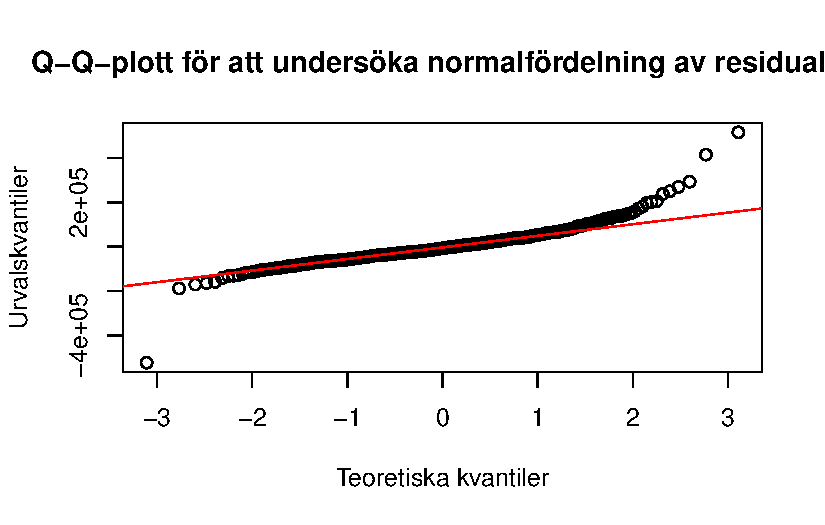
\includegraphics[keepaspectratio]{undersokning_antaganden_files/figure-pdf/unnamed-chunk-3-1.pdf}}

}

\caption{Observationerna följer normalfördelningen väl kring
medelvärdet, men det finns avvikelser i svansarna.}

\end{figure}%

Observationerna följer normalfördelningen väl kring medelvärdet, men det
finns avvikelser i svansarna -- särskilt bland höga värden. Detta
indikerar att man bör vara försiktig vid prediktion av ovanligt höga
bilpriser.

\subsection{Korrelerade residualer
(tidsberoende)}\label{korrelerade-residualer-tidsberoende}

Eftersom datan inte är tidsserier och varje bil är en fristående
observation fanns inget behov av att undersöka tidsberoende residualer.

\subsection{Outliers och leverage}\label{outliers-och-leverage}

\begin{figure}[H]

{\centering \pandocbounded{\includegraphics[keepaspectratio]{undersokning_antaganden_files/figure-pdf/unnamed-chunk-4-1.pdf}}

}

\caption{Leverage-värden för varje observation i modellen.}

\end{figure}%

\begin{verbatim}
[1] 0.3365043
\end{verbatim}

\begin{verbatim}
     price  seller   fuel    gear miles year_model type         wheels hpower
393 389900 Företag Hybrid Automat 12209       2022  SUV Fyrhjulsdriven    350
    engine brand model
393   1969 Volvo  XC60
\end{verbatim}

Leverage-analysen visade att en observation (en hybrid-SUV från 2022 med
350 hk) hade ovanligt stort inflytande på modellen. Då observationen
representerar verkliga och möjliga framtida biltyper valdes den ändå att
behållas i datan.

\subsection{Multikollinearitet}\label{multikollinearitet}

\begin{verbatim}
               GVIF Df GVIF^(1/(2*Df))
fuel       2.991407  4        1.146791
year_model 2.579609  1        1.606116
miles      2.251292  1        1.500431
hpower     2.823176  1        1.680231
\end{verbatim}

Alla prediktorer hade VIF-värden under 3, vilket innebar att det inte
fanns någon allvarlig multikollinearitet i modellen.

\bookmarksetup{startatroot}

\chapter{Slutsatser}\label{slutsatser}

Redan efter första modellträningen uppnåddes ett av målen i arbetet --
att nå en förklaringsgrad R² på minst 0,80. Den första modellen gav ett
R² på över 0,91, vilket visade att en linjär regressionsmodell har
potential att prediktera bilpriser med hög precision.

Nästa fråga var om man kunde nå en liknande förklaringsgrad med färre
prediktorer. Jag undersökte aldrig specifikt om två prediktorer räckte
för att nå R² \textgreater{} 0,80, men jag testade två enklare modeller:
en med tre prediktorer och en med fyra. Båda nådde målet. Resultatet
visade att en modell med endast year\_model, miles, hpower -- och i det
ena fallet även fuel -- kunde prediktera priset på en bil med relativt
hög noggrannhet.

Även om modell 1 presterade bäst rent statistiskt, visade både modell 2
och 3 att det går att nå en förklaringsgrad över 80\,\% utan att använda
alla variabler. Därmed uppnåddes studiens syfte: att ta fram en enkel
men träffsäker modell för att prediktera bilpriser.

\bookmarksetup{startatroot}

\chapter{Teoretiska frågor}\label{teoretiska-fruxe5gor}

Här kan du besvara de frågor som tillhör den teoretiska delen av
uppgiften.

\begin{enumerate}
\def\labelenumi{\arabic{enumi}.}
\item
  En QQ-plot är en graf som visar hur kvantilerna i en datamängd (Y)
  förhåller sig till kvantilerna från en teoretisk fördelning (X),
  oftast en normalfördelning. Om punkterna i grafen följer en ungefärlig
  rak linje, tyder det på att datan är normalfördelad.
\item
  När vi använder en modell för att prediktera så är syftet att få ett
  resultat, exempelvis hur mycket ett hus kan vara värt, vi är då
  intresserade av att få ett värde. När vi talar om inferens så innebär
  det att vi också vill förstå vad det är som påverkar huspriset, och
  således inte bara prediktionen.
\item
  Skillnaden mellan konfidensintervall och prediktionsintervall är att
  prediktionsintervallet är mer osäkert därför att det också inkluderar
  feltermen (slumpmässigheten) epsilon vid en ny observation. Det vill
  säga osäkerheten i själva obeservationen. Därför är
  prediktionsintervallet bredare än konfidensintervallet, som endast
  uppskattar hur säkra vi är på det förväntade medelvärdet Y.
\item
  Beta 0 är interceptet och visar vad \(Y\) skulle vara om alla andra
  variabler är noll. Varje annan beta-parameter (β1 \ldots{} βp) visar
  lutningen för sin respektive variabel. Alltså hur mycket \(Y\)
  påverkas när just den variabeln ändras, medan övriga är konstanta.
  Alla beta tillsammans med feltermen epsilon ger det estimerade värdet
  på \(Y\).
\item
  Man kan använda BIC för att jämföra modeller, men det baseras helt på
  träningsdatan. Det betyder att vi inte får någon riktig uppfattning om
  hur väl modellen fungerar på ny data.
\end{enumerate}

Syftet med att dela upp i träning, validering och test är just att testa
hur modellen generaliserar. Detta är inte något som BIC gör. BIC är ett
hjälpmedel för att välja mellan olika modeller, men det ersätter inte
behovet av att utvärdera modellen på ny data.

\begin{enumerate}
\def\labelenumi{\arabic{enumi}.}
\setcounter{enumi}{5}
\tightlist
\item
  \begin{enumerate}
  \def\labelenumii{\arabic{enumii}.}
  \tightlist
  \item
    Börjar med en modell utan några prediktorer alls. Den estimerar
    medelvärdet för alla observationer.
  \item
    För varje antal prediktorer, från 1 till det totala antalet, testas
    alla möjliga kombinationer av just det antalet prediktorer. Av dessa
    väljs den modell som har bäst resultat. Lägst RSS eller högst R².
  \item
    Slutligen jämförs de bästa modellerna från varje nivå och man väljer
    den av dem baserat på ett utvärderingsmått som BIC, AIC eller
    justerat R². Alternativt genom valideringsdata eller
    cross-validation.
  \end{enumerate}
\item
  Hur bra vi än tränar en modell så kommer den aldrig att vara helt
  korrekt. Den förenklar verkligheten och kommer alltid att ha vissa
  fel. Men om modellen ändå är tillräckligt bra på att prediktera eller
  förklara det vi är intresserade av, kan den fortfarande vara väldigt
  användbar.
\end{enumerate}

\bookmarksetup{startatroot}

\chapter{Självutvärdering}\label{sjuxe4lvutvuxe4rdering}

\begin{enumerate}
\def\labelenumi{\arabic{enumi}.}
\item
  Vad tycker du har varit roligast i kunskapskontrollen? Låter kanske
  diplomatiskt, men jag skulle säga helheten, att det varit flera olika
  moment som jag fått utföra och bygga samman. Att hämta data via API,
  samla in data från Blocket och hanterat svårigheterna i det. Att jag
  verkligen, som jag önskat mer av, få djupdyka i EDAn för att titta på
  datan och hantera saknade värden m.m. Jag tycker också det varit
  givande att få tillämpa mer av den statistiska delen i arbetet för att
  få en djupare förståelse för det och att det faktiskt är häftigt, att
  man vid prediktion eller liknanande också statistiskt genom konfidens-
  och prediktionsintervall kan säga hur ``säker'' man är på det värdet.
  Det tycker jag är väldigt intressant.
\item
  Hur har du hanterat utmaningar? Vilka lärdomar tar du med dig till
  framtida kurser? När jag stött på utmaningar så har jag försökt se
  objektivt på det, alternativt så har jag varit intresserad av att
  undersöka en väg och därför valt att pröva den. Det har inte alltid
  varit tydligt vilken väg man skall gå eller hur ett problem skall
  lösas. Har jag inte direkt kunnat lösa det så har jag lämnat datorn
  ett tag och kommit tillbaka och då fått nya infallsvinklar vilket
  hjälpt mig lösa problemen.
\end{enumerate}

Vidare har jag också när jag hamnat vid ett vägskäl valt att gå den väg
jag vill och tänkt att jag bara argumenterar för min sak och därmed
kommit vidare. Att välja sin väg och argumentara för det tror jag har
varit den mest givande erfarenheten. Allt är långt ifrån perfekt och
problem uppstår och man får omvärdera.

\begin{enumerate}
\def\labelenumi{\arabic{enumi}.}
\setcounter{enumi}{2}
\item
  Vilket betyg anser du att du ska ha och varför? Jag anser mig uppnå de
  kriterier som krävs för VG då jag bland annat tillämpat insamling av
  data via API och insamling av data bia Blocket. Vidare har jag också
  pröva olika modeller, tittat på olika teoretiska antaganden,
  multikollinearitet, linjärt samband mellan X och Y, normalfördelade
  residualer osv. Jag har också metodiskt och mer djupgående granskat
  och hanterat datan och de problem som varit. Tycker att jag gjort ett
  ganska gediget arbete.
\item
  Något du vill lyfta till Antonio? Kursen har varit bra och rolig.
  Gillar som nämnnts ovan att vi fått nyttjat flera olika moment och
  bygga en helhet och att statistiken involverats. Varit väldigt
  lärorikt att undersöka de olika teroretiska antagandena. Du har också
  som vanligt varit väldigt hjälpsam och duktig på att förklara svåra
  begrepp och visa oss hur det fungerar och hänger ihop. Uppskattat!
\end{enumerate}

\bookmarksetup{startatroot}

\chapter{Appendix A}\label{appendix-a}

All kod med mera som använts i detta arbete går att finna på följande
länk: \url{https://github.com/lantzpeter/06_R}

\section{API}\label{api}

Kod för API finns på följande länk
\url{https://github.com/lantzpeter/06_R/api}

\bookmarksetup{startatroot}

\chapter{Referenser}\label{referenser}

Blocket AB. (2024). Blocket -- Sveriges största marknadsplats. Hämtad
från \url{https://www.blocket.se}

Fox, J., \& Weisberg, S. (2023). Companion to Applied Regression (R
package version 3.1-2). \url{https://CRAN.R-project.org/package=car}

Fellows, I. (2020). Metrics: Evaluation Metrics for Machine Learning (R
package version 0.1.4). \url{https://CRAN.R-project.org/package=Metrics}

Hester, J., \& Wickham, H. (2023). glue: Interpreted String Literals (R
package version 1.6.2). \url{https://CRAN.R-project.org/package=glue}

James, G., Witten, D., Hastie, T., \& Tibshirani, R. (2023). An
Introduction to Statistical Learning: with Applications in R (2nd ed.).
Springer. \url{https://www.statlearning.com/}

Lahti, L., \& Nieminen, M. (2024). Accessing PX-Web Statistics from R
with the pxweb Package. Hämtad från
\url{https://ropengov.github.io/pxweb/articles/pxweb.html}

Lumley, T. (2022). Regression Subset Selection (R package version 3.1).
\url{https://CRAN.R-project.org/package=leaps}

OpenAI. (2024). ChatGPT (Version 4.0). \url{https://chat.openai.com}

Posit. (2024). Quarto -- Scientific and Technical Publishing System.
\url{https://quarto.org/}

Prgomet, A. (2024). DS24 R-kursmaterial. Hämtad från
\url{https://github.com/AntonioPrgomet/ds24_r}

Prgomet, A. (2024). R: Validera och jämföra modeller med valideringsdata
{[}YouTube-video{]}. Hämtad från
\url{https://www.youtube.com/watch?v=NcxMuCG6FS8}

Prgomet, A. (2024). Simple Linear Regression -- Föreläsningsanteckningar
{[}PDF{]}. Hämtad från
\url{https://github.com/AntonioPrgomet/linear_regression/blob/main/f%C3%B6rel%C3%A4sningsanteckningar.pdf}%C3%B6rel%C3%A4sningsanteckningar.pdf}%B6rel%C3%A4sningsanteckningar.pdf}%C3%A4sningsanteckningar.pdf}%A4sningsanteckningar.pdf}%C3%B6rel%C3%A4sningsanteckningar.pdf}%B6rel%C3%A4sningsanteckningar.pdf}%C3%A4sningsanteckningar.pdf}%A4sningsanteckningar.pdf

Statistiska centralbyrån. (2024). Statistikdatabasen. Hämtad från
\url{https://www.scb.se}

Wickham, H. (2016). ggplot2: Elegant Graphics for Data Analysis.
Springer-Verlag New York. \url{https://ggplot2.tidyverse.org}

Wickham, H., \& Cetinkaya-Rundel, M. (2023). R for Data Science (2nd
ed.). O'Reilly Media. \url{https://r4ds.hadley.nz}

Wickham, H., et al.~(2023). The tidyverse: Easily Install and Load the
`Tidyverse' (R package version 2.0.0). \url{https://www.tidyverse.org}




\end{document}
